%\paragraph{$R_0$ definition}
%
We calculate the basic reproductive number for lockdown-vaccination model
in \cref{eqn:vacination_dynamics} and present figures with different level
curves of $R^{L,V}_0$. We use van den Driessche's
\cite{VandenDriessche2017a} definition of basic reproductive number. This
threshold parameter means as the average number of secondary cases produced
by an infected individual introduced into a susceptible population.
%
The basic reproductive number $R_0$ for model in \cref{eqn:base_dynamics} is
%
\begin{equation*}\label{eqn:reproductive_number}
    \begin{aligned}
        R_0 :=
        &
            \frac{\kappa}{\kappa + \mu}
            \left[
                \frac{p\beta_S}{R_1}
                + \frac{(1 - p) \beta_A}{\gamma_A+\mu}
            \right],
        \\
        \text{where}
        &
        \\
        R_1 &= \mu + \delta_H + \gamma_S + \mu_{I_{S}}.
    \end{aligned}
\end{equation*}
%
    Note that $p\beta_S/R_2$ measures the proportion of new infections generated
by a symptomatic infectious individual.
Similarly, $(1 - p) \beta_A / (\gamma_A+\mu)$
estimates the new infections generated by an asymptomatic infectious individual.
$(\mu R_1 + \delta_L) / (\delta_L + \mu)$ determines the number of individuals
in lockdown that leave them it, and are infected. Finally,
$\kappa /(\kappa + \mu)$ measures the time of the disease's incubation.

    In the absence of lockdown, our model in
\cref{eqn:vacination_dynamics} has the following basic reproductive number
%
\begin{equation*}
    \label{eqn:reproductive_numberLockdown}
    \begin{aligned}
        R^{L}_0 :=
        &
        \left[
            1 -
            \frac{(1 - \epsilon) \theta \mu}{\delta_L + \mu}
        \right] R_0.
    \end{aligned}
\end{equation*}
%
The first term of $R^{L}_0$ is called reduction factor, which depends on
lockdown parameters.
Observe that in absence of lockdown individuals, $\theta = 0$, $R^{L}_0$
becomes $R_0$.

    Considering lockdown-vaccination, then the basic
reproductive number of the model \eqref{eqn:vacination_dynamics}  $R_{0}^{L,V}$
results
%
\begin{equation*}\label{eqn:reproductive_numberLV}
    R_{0}^{L, V} :=
        \left[
            \frac{
                \lambda_V (1 - \varepsilon) + \delta_V + \mu
            }{
                \delta_V + \lambda_V +
                \mu
           }
        - \frac{
            (1 - \epsilon) \theta \mu
        }{
            \delta_L + \lambda_V + \mu
        }
        \right] R_0.
\end{equation*}
%
    Now, the reduction factor depends on vaccination parameter, and determines
the proportion of vaccinated individuals that becomes infected individuals.
Also, if there’s no vaccination effect,
$
    R_{0}^{L,V} = R_{0}^{L}
$.
%
\begin{figure*}[tbh]
    \centering
    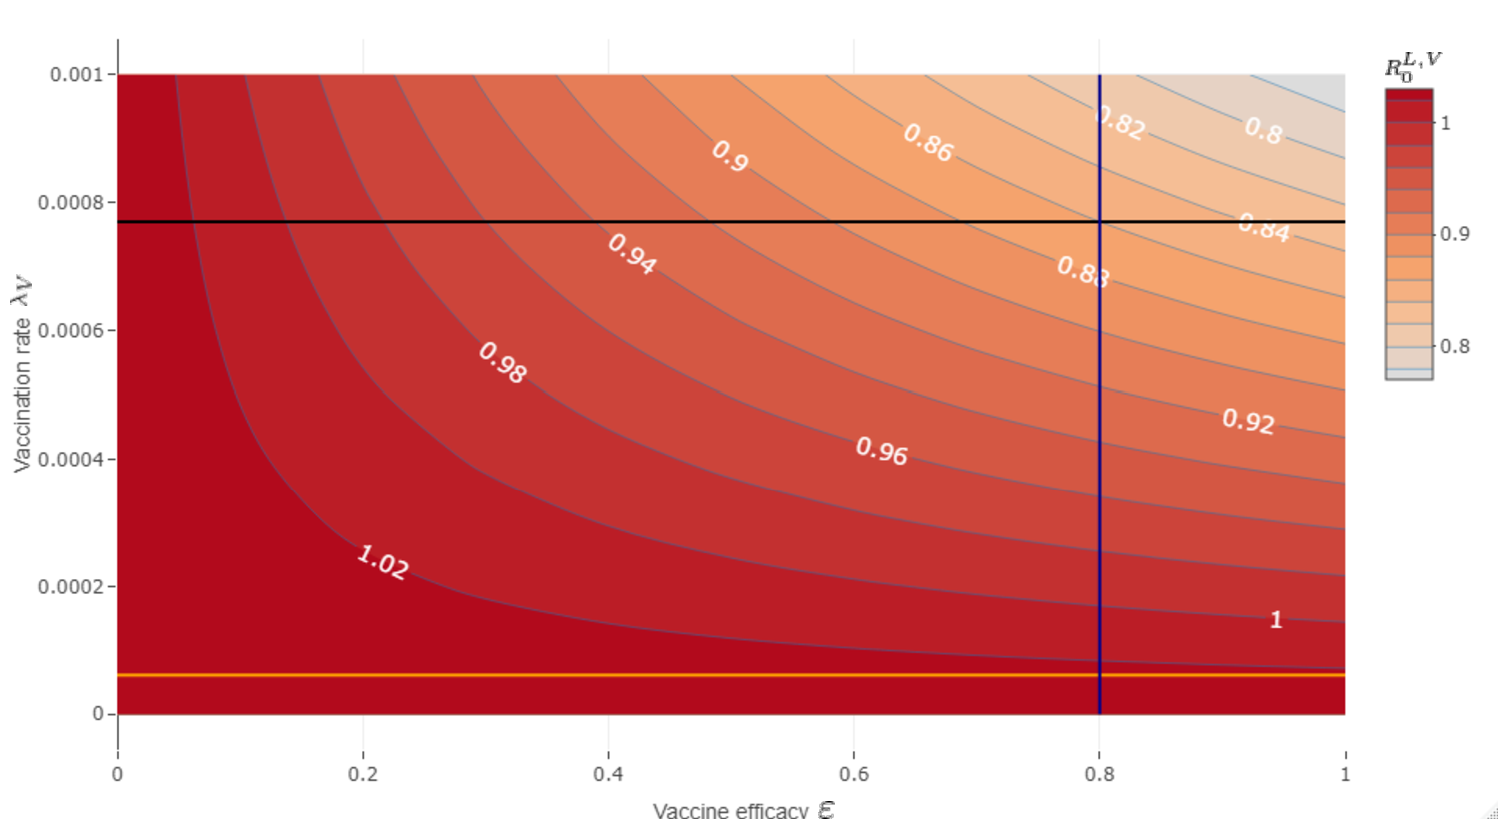
\includegraphics[scale=0.64,keepaspectratio]{./Figures/Rlv_contour.pdf}
    \caption{
        Contour plot of $R_0^{L,V}$ as a function of vaccine efficacy $(
        \varepsilon) $ and vaccination rate $(\lambda_V)$ and vaccine-induced
        immunity average time of one year. The solid orange line represents the
         value of $\lambda_{Vbase}=\num{0.0000611352}$,
        corresponding to a coverage $x_{coverage} = \num{0.2}$ and a horizon
        time $T=\num{365}$ days. The intersection of black line and blue line
        show a scenario in which it is possible to have the $R^{L, V}_0=0.86$,
        considering a vaccine efficacy of $\num{0.8}$ and a vaccination rate of
        $\num{0.0008}$.}
    \label{fig:rvcontour1}
\end{figure*}

\Cref{fig:rvcontour1} displays feasible combinations of vaccination rate and
vaccine
efficacy. In particular,  if we have chosen a vaccination rate below
$\num{0.00025}$
approximately, it is impossible to reduce to $R^{L,V}_0$ below one for any
vaccine
efficacy value. But, taking a vaccination rate greater than $\num{0.0004}$,
it is necessary a vaccine efficacy at least of \SI{50}{\percent} to have
$R^{L,V}_0 < 1$.
%
\begin{figure*}[tbh]
    \centering
    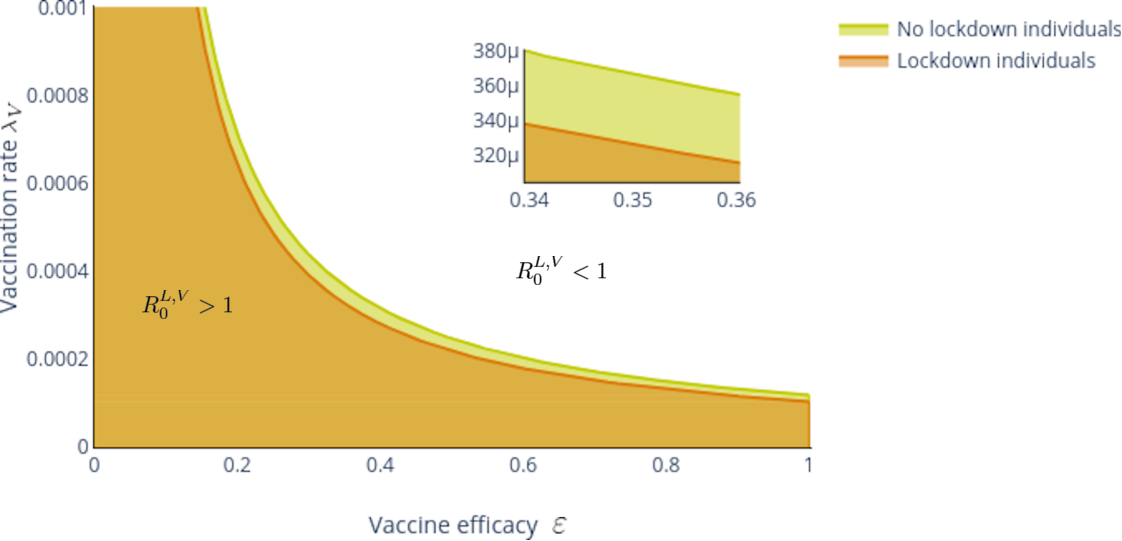
\includegraphics[scale=0.8,
    keepaspectratio]{./Figures/Rlv-feasible-region.pdf}
    \caption{
        Comparison of vaccination feasible region. The color regions show
        $R_0^{L,V}>1$, and white region $R_0^{L,V}<1$. Yellow-shaded region
        represent vaccination feasible region without lockdown individuals,
        orange-shaded region with lockdown individuals
        \href{https://plotly.com/~AdrianSalcedo/85/}{%
            https://plotly.com/~AdrianSalcedo/85/}
    }
    \label{fig:FeasibleRegion}
\end{figure*}
%
    We exhibit vaccination regions, with and without lockdown individuals in
\Cref{fig:FeasibleRegion}. Note that the region to have $R^{L,V}_0<1$ is
greater in the case with lockdown individuals than in the case without lockdown
individuals. For example, fixing a vaccine efficacy of $\num{0.35}$, we need to
vaccinate fewer individuals in the case of lockdown individuals than without
lockdown individuals to get $R^{L,V}_0<1$. And setting a vaccination rate of
$\num{0.00034}$, it is required at least a vaccine efficacy of $\num{0.35}$, in
case with lockdown individuals. But in the case without lockdown individuals, we
require at least $\num{0.36}$. These tell us that, implementing a strategy of
lockdown-vaccination instead of just vaccination reduces the number of
individuals to be vaccinated with less vaccine efficiency.
